%\begin{figure*}[!t]
%	\begin{center}
%		\subfigure[No Failure]
%		{
%			\label{fig:sc_no_fail}
%			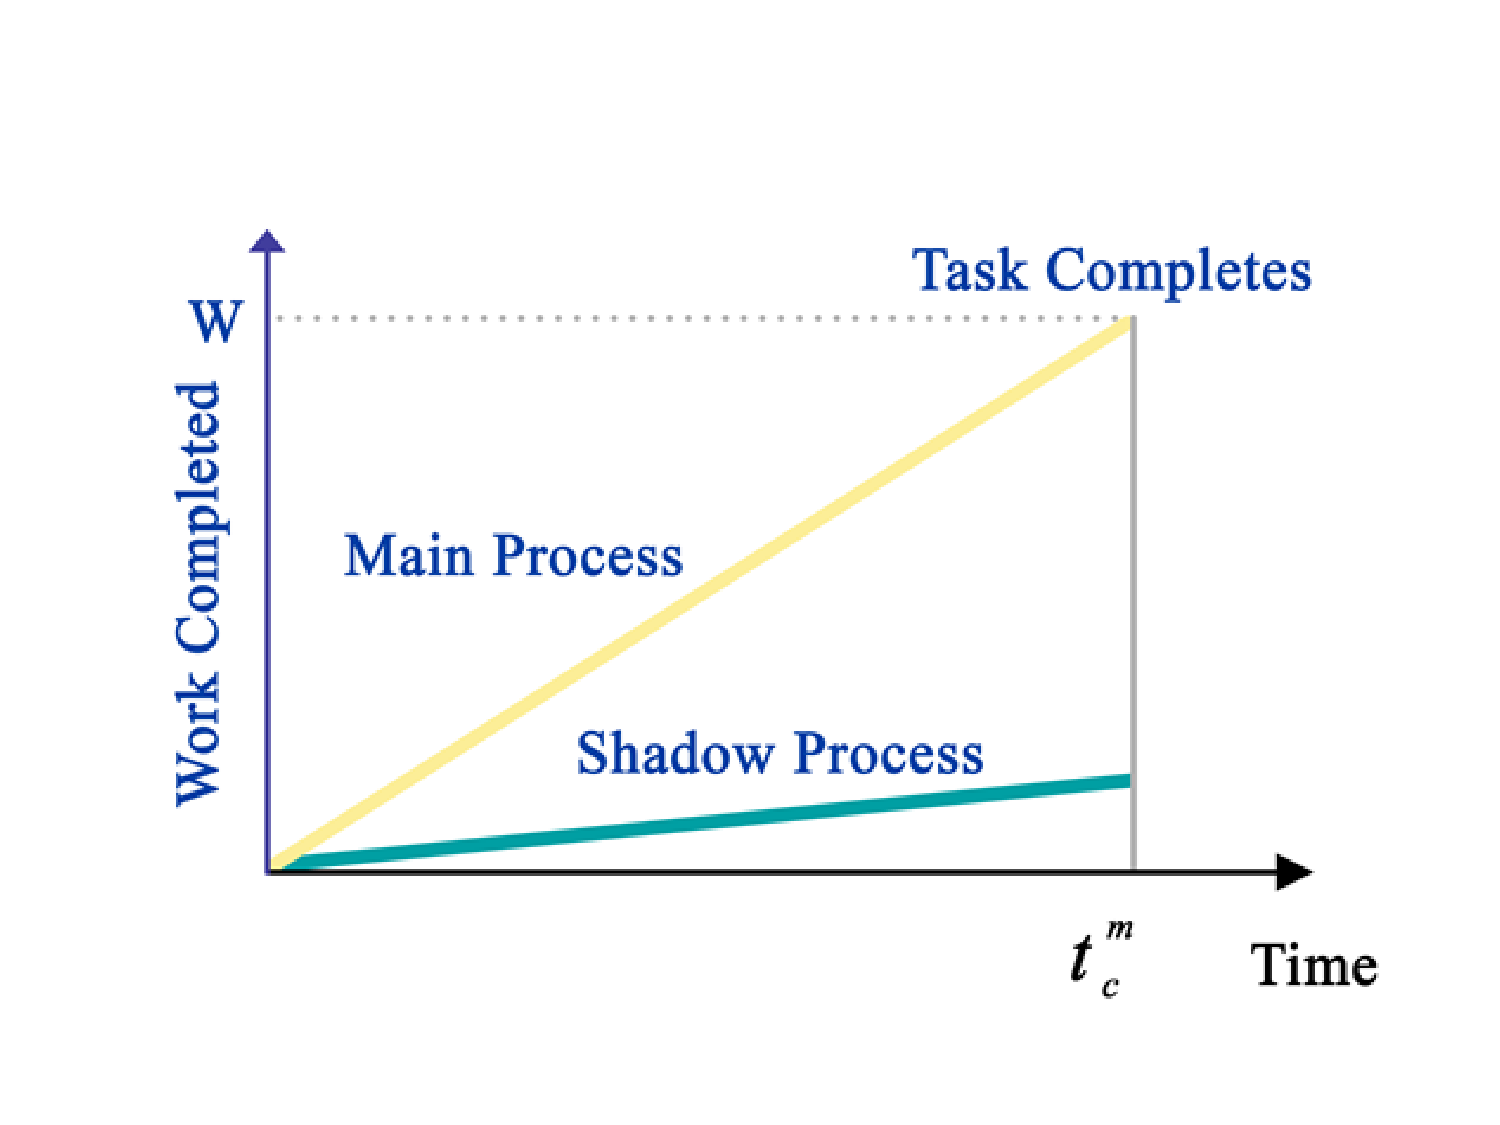
\includegraphics[width=0.32\textwidth]{Figures/example1.pdf}
%		}
%		\subfigure[Shadow Process Failure]
%		{
%			\label{fig:sc_shadow_fail}
%			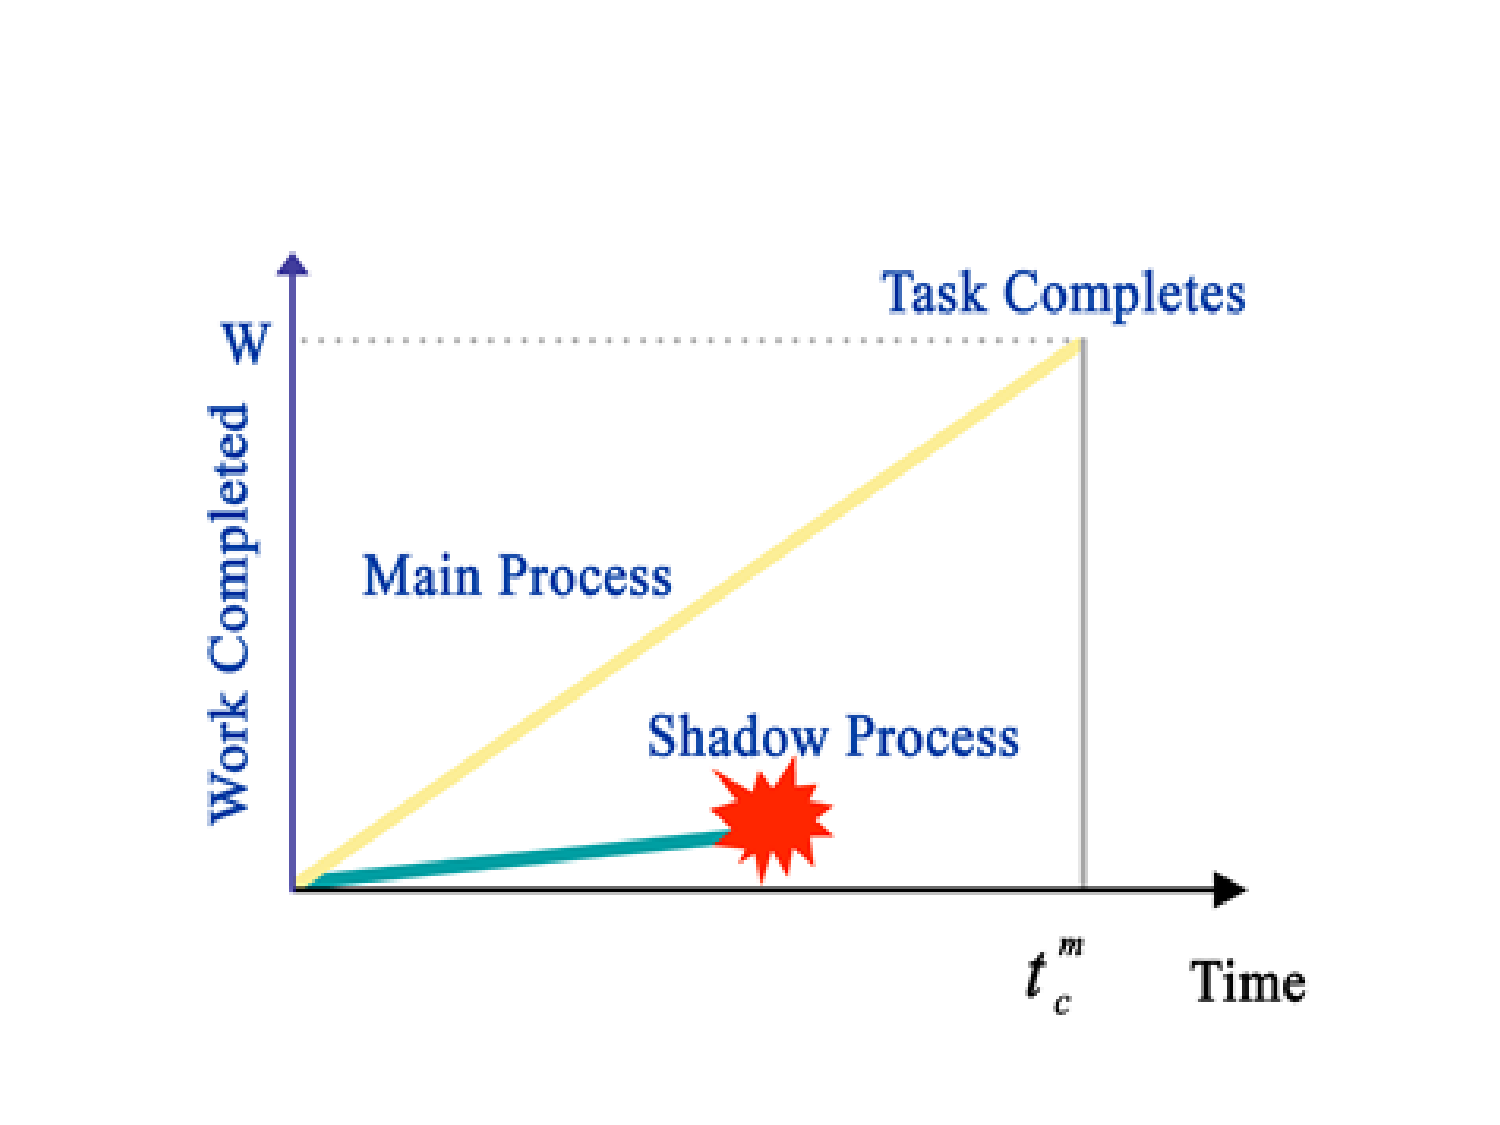
\includegraphics[width=0.29\textwidth]{Figures/example3.pdf}
%		}
%		\subfigure[Main Process Failure]
%		{
%			\label{fig:sc_main_fail}
%			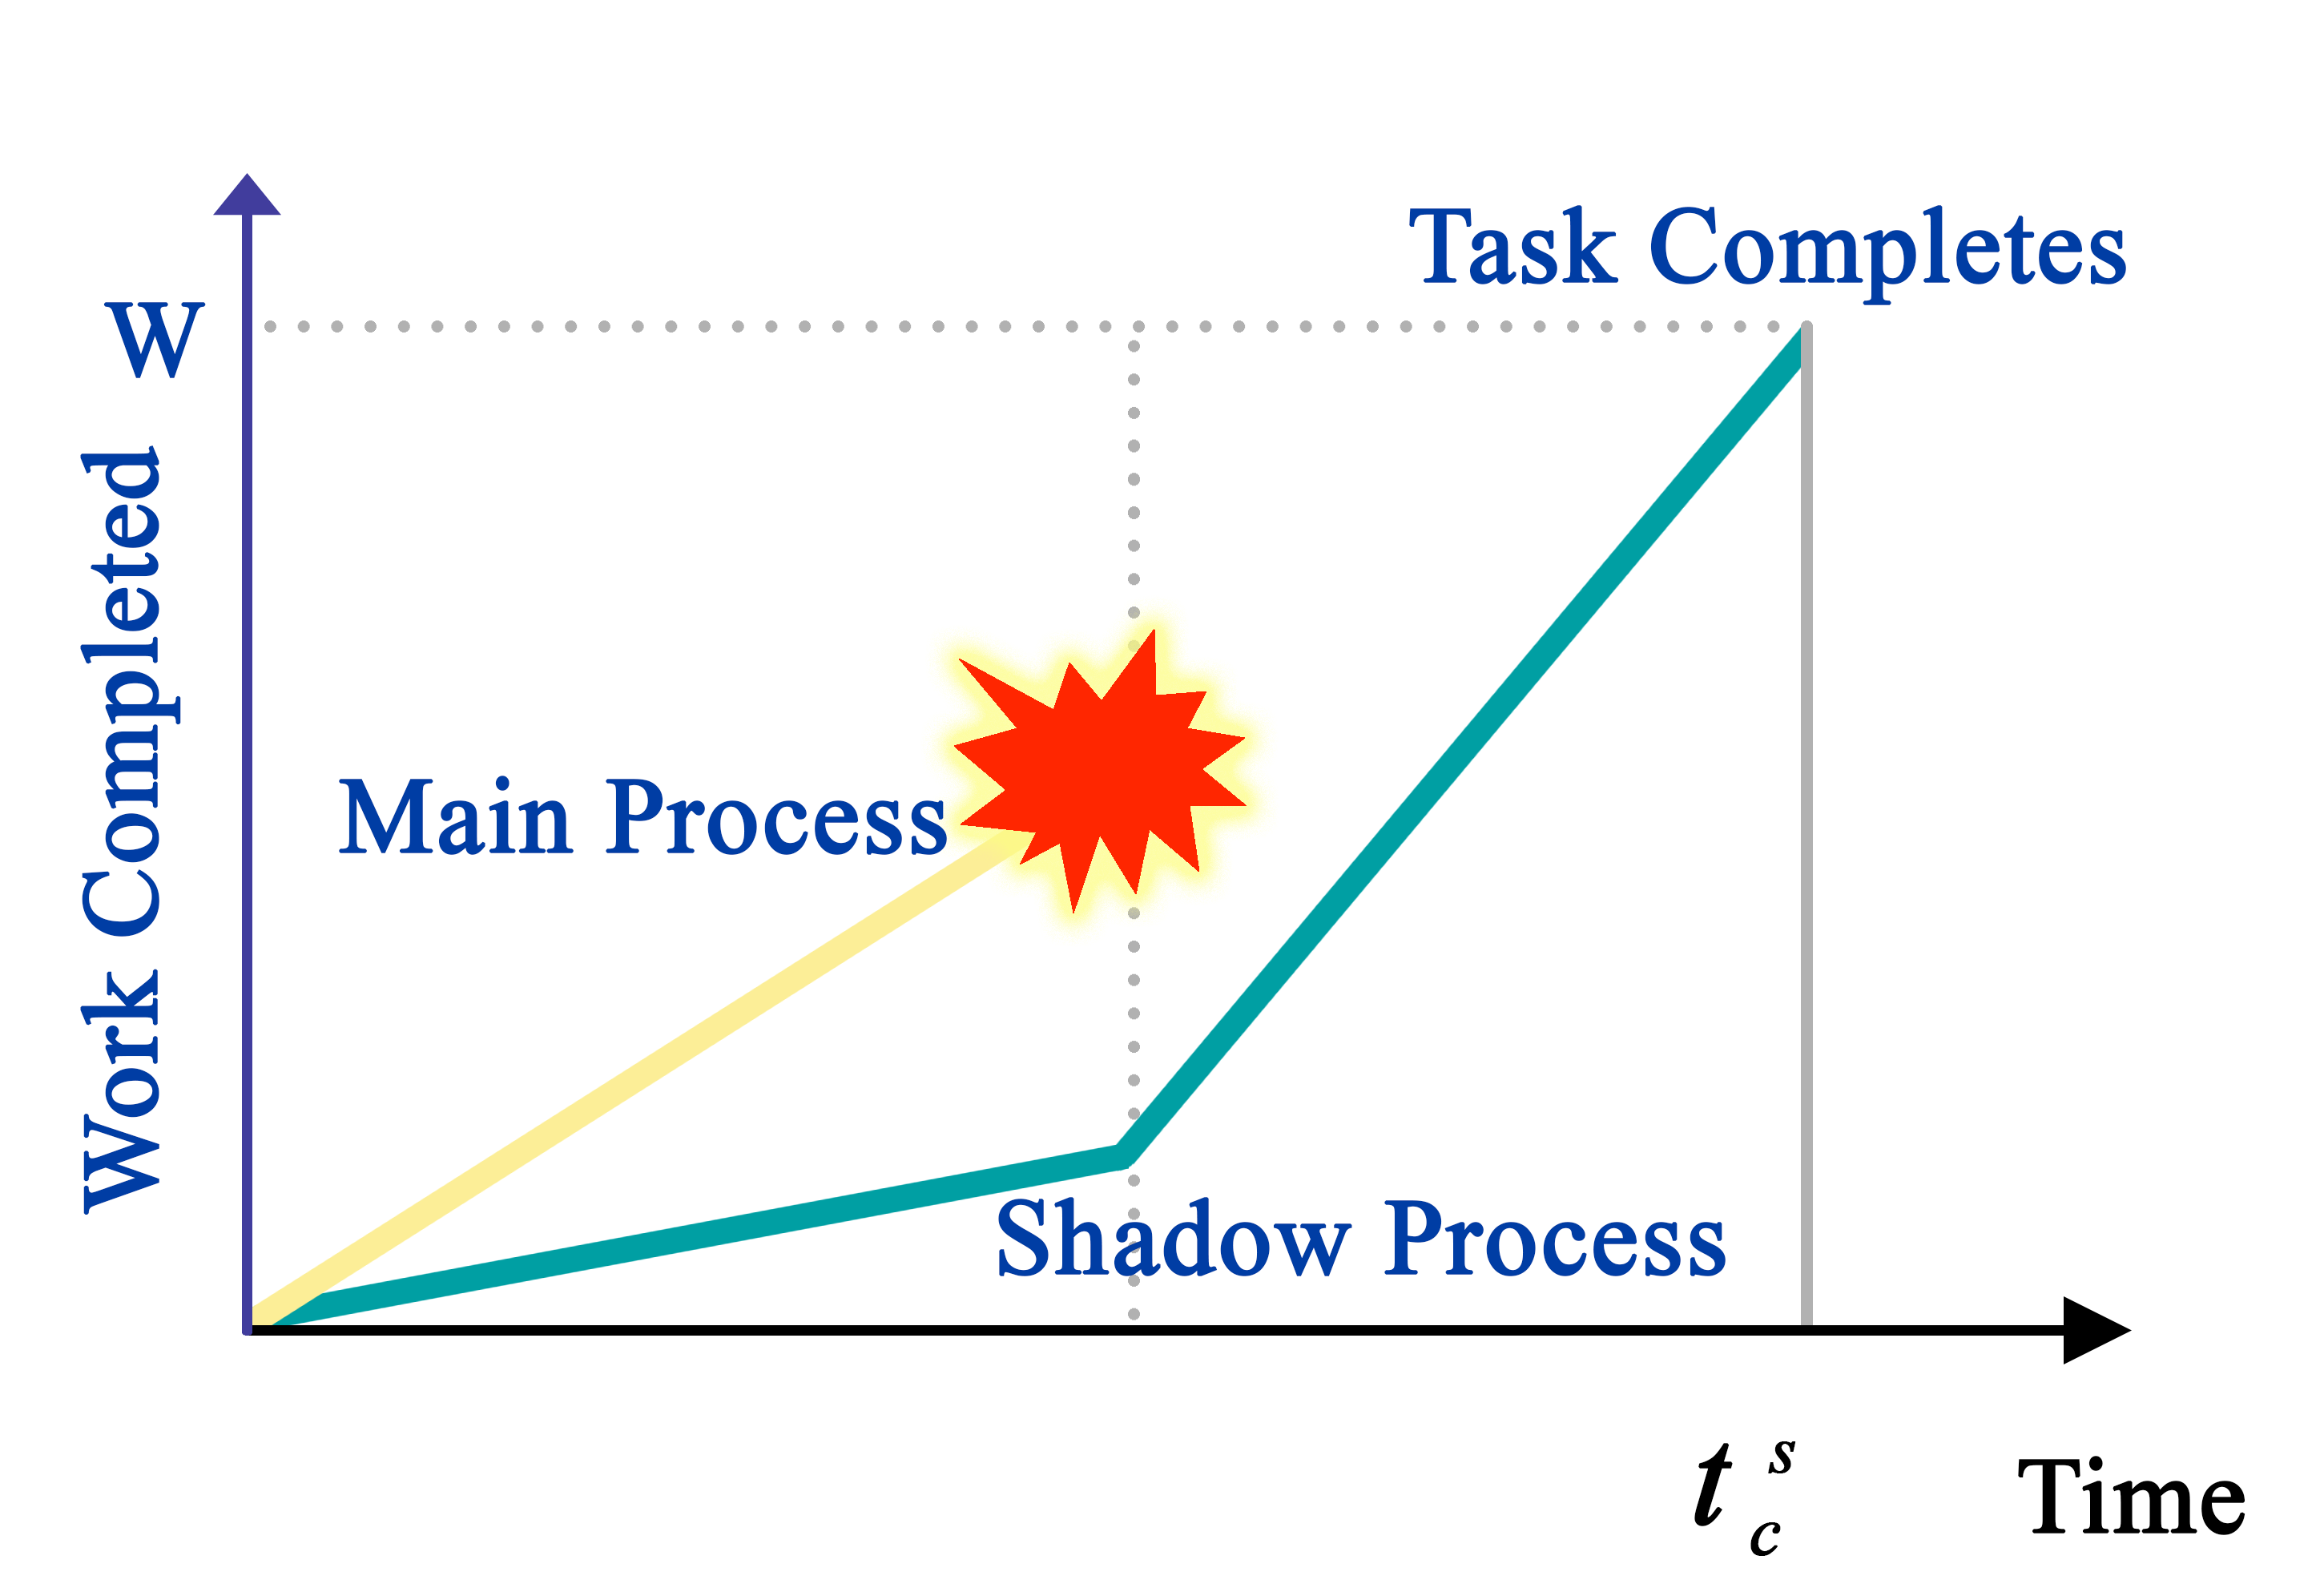
\includegraphics[width=0.33\textwidth]{Figures/example2.png}
%		}
%	\end{center}
%	\caption{Shadow Replication with a single shadow process.}
%	\label{fig:sc_overview}
%	\end{figure*}

The basic tenet of the proposed fault tolerance framework, referred to as Shadow Computing, is to associate with each main execution instance (a process or a thread) a suite of ``shadow instances", whose size depends on the criticality of the application and its performance requirements. 
To mitigate correlated failures, the main and shadow instances
execute on separate computing nodes.

The novelty of Shadow Computing lies in its differentiation of the execution rates. Specifically, it 
executes the main instance at the rate required for response time constraint, while slowing down the shadows for energy saving, thereby enabling a parameterized trade-off between response time and energy consumption.
Shadow Computing is a generalization of existing fault tolerance
approaches. %, namely Checkpoint/restart and Process Replication. 
Specifically, if there is enough laxity in response time constraint, Shadow
Computing would start the shadows only after the main instance fails, mimicking Re-execution. %It is clear, therefore, that for a
%large response time, Shadow Replication converges to re-execution, as
%the shadow remains idle during the execution of the main process and
%only starts execution upon failure. 
If the target response time is
stringent, however, %Shadow Replication converges to process replication,
the shadows would execute simultaneously with the main at the maximal
rate, mimicking Process Replication. The flexibility of Shadow Replication provides a spectrum
of fault tolerance strategies that strike a
balance between completion time and energy saving.


\subsection{Execution rate control}
One challenge in Shadow Computing is how to control the execution rates. So far, we have explored two methods to differentiate the execution rates among the instances. The first approach is to use Dynamic Voltage and Frequency Scaling (DVFS), of which the CPU frequency (execution rate) scales linearly with the supply voltage and the power consumption has a super-linear relationship with the frequency~\cite{cui_en7085151,cui_closer_2014}. Our second approach is to use time sharing to reduce the effective execution rate while keeping the computing nodes running at maximal frequency. Since this approach collocates multiple execution instances on a same node, it reduces the number of machines to be used and the energy consumption correspondingly~\cite{cui_ics_2015}.

\subsection{Modeling and Simulation}
The other challenge resides in determining
jointly the execution rates of all processes, %both before and
%after a failure occurs, 
with the objective to minimize energy while satisfying QoS requirements. To achieve this, I propose two analytical
models, corresponding to the two rate-control approaches above. The models consider the time and energy needed for a job, %which is composed of multiple parallel tasks, 
under different system specifics and failure distributions. From the analytical models an optimization problem is formulated and solved to derive the optimal execution rates.  %The profit is modeled as the difference between the payment from customers, which depends on the completion time, and expenses for running the cloud job, which are mainly energy costs. %Afterwards, an optimization problem is formulated to derive the optimal execution rates. 
%For more details please refer to~\cite{cui_en7085151}. 

To verify the correctness of the analytical models, I build an event-driven simulator that simulates the behaviors of Shadow Computing under different system specifics, task characteristics, and failure distributions. It can report all necessary statistics, such as number of failures encountered, time to completion, and energy consumption. The statistics can then be used to compare with the results from the analytical model.

\subsection{Results}
Several important parameters are identified that impact the energy consumption of Shadow Computing. Correspondingly, I conduct a series of sensitivity studies where Shadow Computing is compared to state-of-the-art approaches. %The influential parameters can be classified into three categories, i.e., system specifics, SLA specifics, and job specifics. Further, the system specifics includes static power/dynamic power ratio and failure distribution, the job specifics includes workload and number of tasks, and SLA specifics is mainly targeted job completion time 
The results from both the analytical model and simulator show that Shadow Computing can achieve significant energy savings, without violating the QoS constraints. %Specifically, I conducted 4  sensitivity studies. 
Specifically, Shadow Computing can achieve 15\%-30\% energy savings under normal configurations. Furthermore, Shadow Computing would converge to Process Replication, when target response time is stringent, and to Re-execution when target response time is relaxed or when failure is unlikely.%~\cite{cui_closer_2014}.




